\documentclass[12pt]{article}
\usepackage{listings}
\usepackage{amsmath}
\usepackage[pdftex]{graphicx}
\usepackage{fancyvrb}
\usepackage{chapterbib}
\usepackage{hyperref}
\usepackage{wrapfig}
\usepackage{subfig}

\pdfcompresslevel=9
\DeclareGraphicsExtensions{{.png},{.pdf},{.jpg},{jpeg}}
\graphicspath{ {../figures/}}
\usepackage{color}

\hypersetup{%
  bookmarksnumbered, pdftitle={Uintah Installation Guide},
  pdfauthor={John Schmidt, Todd Harman, James Sutherland,
    Jeremy Thornock, J. Davison de St. Germain, Tony Saad},
  pdfsubject={Installation Guide}, pdfkeywords={Uintah}, pdfview=FitH,
  pdfborder=0 0
  0, % make all links invisible, so the pdf looks good when printed
  pdffitwindow=false, % window fit to page when opened
  pdfstartview={FitH}, % fits the width of the page to the window
  pdfnewwindow=true, % links in new window
  colorlinks=true, % false: boxed links; true: colored links
  linkcolor=blue, % color of internal links
  citecolor=darkred, % color of links to bibliography
  filecolor=darkred, % color of file links
  urlcolor=magenta % color of external links
}
%__________________________________
% new commands for all sections --- !!!! FIXME: This should be pulled in from
% user_guide.tex... not sure how to do this !!!!
\newcommand{\TT}[1]{\tt{#1} \normalfont}

\begin{document}

\title{Uintah Installation Guide}

\author{John Schmidt, Todd Harman, Jeremy Thornock, \\
  James Sutherland, J. Davison de St. Germain, Tony Saad}

\date{Version 2.0}

\maketitle



\newpage

\tableofcontents

\newpage

\section{Overview of Uintah} \label{sec:overview} The \textbf{Uintah}
library is composed of several executables and a generic library
framework for solving PDEs on structured AMR grids on large parallel
supercomputers. \textbf{\emph{VisIt}} is used to visualize data
generated from \textbf{Uintah}.

\subsection{Obtaining the Code}
Uintah can be obtained either as a compressed tarball from
\url{http://www.sci.utah.edu/uintah-survey.html} or by
using Subversion (SVN) to download the latest source code:

\begin{verbatim}
svn co https://gforge.sci.utah.edu/svn/uintah/trunk uintah
\end{verbatim}

The above command checks out the \textbf{Uintah} source tree and
installs it into a directory called uintah in the users home
directory.


\section{Installation Overview}

\textbf{Uintah} can be installed individually and in conjunction with
the visualization tool, \textbf{\emph{VisIt}}.  \textbf{\emph{VisIt}}
has the Uintah database reader included in the build\_visit scripts.

The installation procedure follows the basic outline:

\begin{enumerate}

\item Install basic dependencies: MPI, Blas, Lapack, Hypre, PETSc,
  Boost, \emph{etc}.

\item Configure Uintah

\item Compile Uintah

\item Install visualization tools (optional if installing on a
  supercomputer or first time users).


\end{enumerate}



\section{Generic Library Dependencies}

\textbf{Uintah} depends on several different libraries that are
commonly available or easily installable on various Linux or Unix like
OS distributions.

Required libraries:
\begin{itemize}
\item mpi (OpenMpi, Mpich, or LAM or a vendor supplied mpi library)
\item blas
\item lapack
\item make
\item libxml2-devel
\item zlib-devel
\item c++
\item fortran
\item subversion
\item cmake (version 3.1.0 or higher) -- \textbf{Required for Arches/Wasatch}
\item git
\item boost (version 1.54 or higher) -- \textbf{Required for Arches/Wasatch}
\item Hypre (version 2.9.0b or higher) -- \textbf{Required}
\item PETSc (version 3.5.2 or higher) -- \textbf{Optional}
\end{itemize}


\section{OS Version Dependencies}
\label{sec:dependencies}
\subsection{Debian \& Ubuntu Dependencies}
\label{sec:debian_dependencies}
The \textbf{Gnu/Debian} OS \url{http://www.debian.org} and
\textbf{Ubuntu} OS \url{http://www.ubuntu.org} offer the vast majority
of libraries necessary for installing \textbf{Uintah} with the
exception of VisIt.  Either one of these distributions are
the recommended OS to install.

Installing the following libraries will ensure that all dependencies
required for \textbf{Uintah} are satisfied:

\begin{verbatim} 
sudo apt-get install subversion libhypre-dev petsc-dev \ 
libxml2-dev zlib1g-dev liblapack-dev cmake libglew-dev \
libxmu-dev g++ gfortran libboost-all-dev git \
libxrender-dev libxi-dev
\end{verbatim}

For Debian \textbf{Jessie, version 8}, add the following to
/etc/apt/sources:

\begin{verbatim}
deb http://ftp.debian.org/debian jessie-backports main non-free
contrib
\end{verbatim}

\noindent
then replace an older version of cmake with a newer version of cmake
that is compatible with the Wasatch component. 

\begin{verbatim}
sudo apt-get update
sudo apt-get install -t jessie-backports cmake
\end{verbatim}



\subsection{Fedora Core  Dependencies}

\textbf{Fedora Core 25} \url{http://fedoraproject.org/} offers all the
dependencies except for PETSc and HYPRE.  Install the following
libraries:

\begin{verbatim}
sudo dnf install make openmpi-devel openmpi lapack-devel \
gcc-gfortran blas-devel gcc-c++ libxml2-devel subversion \ 
cmake tar diffutils libX11-devel libXext-devel patch wget \
mesa-libGL-devel mesa-libGLU-devel libXt-devel git boost-devel \
libXrender-devel libXi-devel python qt-devel
\end{verbatim} 

Please see section~\ref{hypre-fedora-centos} for hypre installlation
instructions and section~\ref{petsc-fedora-centos} for petsc installation instructions.



\subsection{CentOS  Dependencies}

\textbf{CentOS 7} \url{http://www.centos.org/} is similar to \textbf{Fedora
Core}.  However, a more recent version of cmake and boost must be installed. 
Please see the sections for install cmake and boost below, along with 
instructions for installing hypre (required) and petsc (optional).

\begin{verbatim}
sudo yum install make openmpi-devel openmpi lapack-devel \
gcc-gfortran blas-devel gcc-c++ libxml2-devel subversion \ 
tar diffutils libX11-devel libXext-devel patch wget \
mesa-libGL-devel mesa-libGLU-devel libXt-devel git \
libXrender-devel libXi-devel bzip2
\end{verbatim} 

\subsubsection{Boost}

Install \textbf{Boost 1.64.0} \url{http://www.boost.org/users/download/}.
After unzipping, then build and install boost:

\begin{verbatim}
cd path/to/boost_1_64_0
./bootstrap.sh
sudo ./b2 install
\end{verbatim}



\subsubsection{CMake}
Install version 3.1.0 or higher of \textbf{CMake} \url{https://cmake.org/download/}

\begin{verbatim}
./bootstrap
  make
  sudo make install
\end{verbatim}

Please see section~\ref{hypre-fedora-centos} for hypre installlation
instructions and section~\ref{petsc-fedora-centos} for petsc installation instructions.


\subsection{OpenSuse  Dependencies}

\textbf{OpenSuse-Leap} \url{http://www.opensuse.org/} is similar to
\textbf{Fedora Core}

\begin{verbatim}
sudo zypper install make openmpi-devel openmpi lapack \
gcc-fortran blas gcc-c++ libxml2-devel subversion \ 
cmake tar diffutils libX11-devel libXext-devel patch wget \
mesa-libGL-devel mesa-libGLU-devel libXt-devel git boost-devel \
libXrender-devel libXi-devel qt-devel glu-devel
\end{verbatim} 

Please see section~\ref{hypre-opensuse} for hypre installlation
instructions and section~\ref{petsc-opensuse} for petsc installation instructions.

\subsection{MacOSX  Dependencies}
Use Macports to install the following:

\begin{verbatim}
sudo port install openssh screen dialog zlib cmake bash autoconf \
                  xmlstarlet gdb gmake
sudo port install mpich
sudo port install mpich-gcc5
sudo port install lapack +gcc5
sudo port select --set mpi mpich-gcc5-fortran
sudo port select --set gcc mp-gcc5
sudo port install -s icu configure.compiler=macports-gcc-5  \
                     configure.cxx_stdlib="libstdc++"
sudo port install -s boost configure.compiler=macports-gcc-5 \
                     configure.cxx_stdlib="libstdc++"
sudo port install -s -v hypre +mpich
\end{verbatim}

You will want to ensure that your path has the macports install
locations before the system ones, i.e., \texttt{/opt/local/bin} before
\texttt{/usr/bin}.



\section{Hypre Installation -- Required}

Hypre can be installed by executing the following simplified
instructions, however, if you encounter problems please refer to the
hypre website for troubleshooting.

Download hypre-2.11.2 from
\url{https://computation.llnl.gov/casc/hypre/software.html}

\subsection{Fedora \& CentOS}
\label{hypre-fedora-centos}
The following configure script assumes the location of MPI libraries
are in \texttt{/usr/lib64/openmpi/lib}.  Note that the
\texttt{LD\_LIBRARY\_PATH} must be set.  It is helpful to include the
\texttt{/usr/lib64/openmpi/bin} in your path for the location of
mpirun and mpiCC, mpicc, and mpif77.


\begin{verbatim}
cd hypre-2.11.2/src

LD_LIBRARY_PATH=/usr/lib64/openmpi/lib/ \
 ./configure --enable-shared \
             --prefix=/usr/local \
             --with-MPI-lib-dirs=/usr/lib64/openmpi/lib/ \
             --with-MPI-include=/usr/include/openmpi-x86_64/ \
             --with-MPI-libs="mpi mpi_cxx" \
             CC=/usr/lib64/openmpi/bin/mpicc \
             CXX=/usr/lib64/openmpi/bin/mpic++ \
             F77=/usr/lib64/openmpi/bin/mpif77

make
sudo make install

\end{verbatim}

\subsection{OpenSuse}
\label{hypre-opensuse}
\begin{verbatim}

cd hypre-2.11.2/src

./configure --enable-shared \
	    --prefix=/usr/local \
            --with-MPI-libs="mpi mpi_cxx" \
            CC=/usr/lib64/mpi/gcc/openmpi/bin/mpicc \
            CXX=/usr/lib64/mpi/gcc/openmpi/bin/mpic++ \
            F77=/usr/lib64/mpi/gcc/openmpi/bin/mpif77

make
sudo make install

\end{verbatim}


\section{PETSc Installation -- Optional}

PETSc can be installed by executing the following simplified
instructions.  Please refer to the PETSc website for comprehensive
installation instructions if you encounter any difficulties.

Download petsc-v3.7.6 from
\url{http://www.mcs.anl.gov/petsc/petsc-as/download/index.html}

\subsection{Fedora \& CentOS}
\label{petsc-fedora-centos}

The following configure script assumes the location of MPI libraries
are in \texttt{/usr/lib64/openmpi/lib}.  Note that the
\texttt{LD\_LIBRARY\_PATH} must be set.  It is helpful to include the
\texttt{/usr/lib/64/openmpi/bin} in your path for the location of
mpirun and mpiCC, mpicc, and mpif77.

\begin{verbatim}
tar zxf petsc-3.7.6.tar.gz
cd petsc-3.7.6

LD_LIBRARY_PATH=/usr/lib64/openmpi/lib \
./configure --with-shared-libraries \
            --with-debugging=0 \
            --with-mpi-dir=/usr/lib64/openmpi/  \
            --prefix=/usr/local

make PETSC_DIR=/home/jas/petsc-3.7.6 PETSC_ARCH=arch-linux2-c-opt all

sudo make install 
\end{verbatim}

\subsection{OpenSuse}
\label{petsc-opensuse}
\begin{verbatim}
tar zxf petsc-3.7.6.tar.gz
cd petsc-3.7.6

./configure --with-mpi-dir=/usr/lib64/mpi/gcc/openmpi \
            --with-shared-libraries --with-debugging=0 \
            --prefix=/usr/local

make PETSC_DIR=/home/jas/petsc-3.7.6 PETSC_ARCH=arch-linux2-c-opt all

sudo make install

\end{verbatim}


\section{Configuring and Building Uintah}

\subsection{Configure}

The following information specifies how to run the ``configure''
script to prepare for building the Uintah executable.  ``Configure''
is a program that checks the computer's environment and looks for the
location of libraries and header files, etc.  When it finishes
running, it will create the \TT{configVars.mk} file which will include
all the information it has determined about the computer.  The
following lines show \textbf{generically} how to use ``configure''.

Goto the directory \TT{ \textasciitilde/uintah} and create the
following directories: \TT{dbg} (debug) and \TT{opt} (optimized)

\begin{verbatim}
cd ~/uintah-2.0
mkdir dbg opt
\end{verbatim}

Go to the \TT{dbg} directory and enter the following:

\begin{verbatim}
../src/configure --enable-debug --enable-all-components \
                 --enable-wasatch_3p --with-boost=[path to boost]
\end{verbatim}


After the configuration process, type \TT{make} to compile Uintah.

If you wish to attach a debugger to Uintah, make sure you use the
\TT{--enable-debug} configure option.

If you would like to reduce the amount of output given by the make
system when making Uintah, you can set the environment variable
\TT{SCI\_MAKE\_BE\_QUIET} to true:

\begin{verbatim}
setenv SCI_MAKE_BE_QUIET true (csh)

export SCI_MAKE_BE_QUIET=true (bash)
\end{verbatim}

Once a debug build has finished, change to the \TT{opt} directory and
enter the following configure line:

\begin{verbatim}
../src/configure '--enable-optimize=-O3 -mfpmath=sse' \
                  --enable-all-components --enable-wasatch_3p \
                  --with-boost=[path to boost]
\end{verbatim}

The debug/optimize flags do the following:  --enable-debug adds ``-g''
to the compile line; --enable-optimize, if used without parameters,
adds ``-O2'' to the compile line.  Otherwise it adds the parameters
specified during configure.

\subsubsection{Other configure options}

Other useful configure options are seen below.  Note, depending on
where libraries are installed on your system, you may or may not need
to specify some (or all) of these options:

By default, Uintah does not build any simulation components (such as
ICE, Arches, Wasatch, or MPM) - though Example components are built.
To turn on components, use the following configure flags:

\begin{verbatim}
--enable-all-components       <= Turns on all simulation components
--enable-arches               <= Turns on Arches
--enable-ice                  <= Turns on ICE
--enable-mpm                  <= Turns on MPM
--enable-mpmice               <= Turns on MPMICE
--enable-wasatch              <= Turns on Wasatch
\end{verbatim}

\begin{verbatim}
--enable-shared               <= Uses shared libraries (Default)
--enable-static               <= Uses static libraries 
--with-mpi=/usr/lib64/openmpi <= Specifies location of MPI
--enable-64bit                <= Specifies a 32 or 64bit build
--enable-32bit
--with-petsc=/path/petsc-3.7.6            <= Specifies location of PETSc
--with-hypre=/path/hypre-2.11.2./hypre_install <= Specifies location of Hypre

F77=gfortran-4.7              <= Specifies compilers (Fortran, C, C++).
CC=/usr/bin/gcc-4.7
CXX=/usr/bin/g++-4.7
PETSC_ARCH=linux-gnu-c-real-opt <= Specifies PETSc architecture

        --without-fortran     <= Turns off the use of Fortran. (Only
useful if you are not building Arches and you do not have a working
Fortran compiler on your computer. 

\end{verbatim}

Arches requires the Wasatch component to be enabled, therefore to
compile the Arches and Wasatch components add:
\begin{verbatim}
  --with-wasatch --with-boost=<path to boost install>, e.g. /usr
  --enable-wasatch_3p
\end{verbatim}
to the configure line.

To see a full list of all the configure options type:

\begin{verbatim}
    ../src/configure --help
\end{verbatim}

\subsubsection{Common Configure Lines}

\paragraph{Debian \& Ubuntu}
\begin{verbatim}
    ../src/configure --enable-debug --enable-all-components \
                     --with-boost=/usr --enable-wasatch_3p F77=gfortan
\end{verbatim}


\paragraph{Fedora \& CentOS}
\begin{verbatim}
../src/configure --enable-debug --enable-all-components \
                 --with-mpi-lib=/usr/lib64/openmpi/lib \
                 --with-mpi-include=/usr/include/openmpi-x86_64 \
                 --with-boost={/usr,/usr/local} --enable-wasatch_3p \
                 --with-hypre=/usr/local 
                 --with-petsc=/usr/local
\end{verbatim}


\paragraph{OpenSuse}
\begin{verbatim}
../src/configure --enable-debug --enable-all-components \
                 --with-mpi-lib=/usr/lib64/openmpi/lib \
                 --with-mpi-include=/usr/include/openmpi-x86_64 \
                 --with-boost=/usr --enable-wasatch_3p \
                 --with-hypre=/usr/local
                 --with-petsc=/usr/local
\end{verbatim}

\paragraph{MacOSX}
\begin{verbatim}
../src/configure --enable-debug --enable-all-components \
                 --with-boost=/opt/local --enable-wasatch_3p \
                 --with-hypre=/opt/local --with-lapack=/opt/local \
                 --with-zlib=/opt/local  \
                 CXX=mpicxx CC=mpicc F77=mpif77

\end{verbatim}


\subsection{Build}

Then build the software by typing \TT{make} at the command line and create symbolic links to the inputs directory found in \TT{\textasciitilde/uintah/src/StandAlone/inputs}.
\begin{verbatim}
   make
\end{verbatim}


Please see the \textbf{User Guide}
\url{http://www.uintah.utah.edu/trac/chrome/site/uintah.pdf} on how to use
the various tools and executables within the \textbf{Uintah}
framework.


\section{Installing VisIt}

Visualization of \textbf{Uintah} data is currently possible using
\textbf{\emph{VisIt}}. The VisIt package from LLNL is general purpose
visualization software that offers all of the usual capabilities for
rendering scientific data.  It is still developed and maintained by
LLNL staff, and its interface to \textbf{Uintah} data is supported by
the Uintah team.

\textbf{\emph{VisIt}} may be downloaded from the following \url{https://wci.llnl.gov/simulation/computer-codes/visit/executables}.

\subsection{VisIt Installation}

The latest official release of \textbf{\emph{VisIt}} is 2.12.2
However, the instructions apply to earlier versions such as 2.12.X.
Using the build\_visit script along with the \emph{--uintah} option,
UDA reader plugin can be built.  \textbf{\emph{VisIt}} can be
installed either from one of their binary distributions, or by
compiling and installing it from source.  You may also need to build
\textbf{\emph{VisIt}} from source (using the build\_visit script) if a
binary is not provided for your exact OS and MPI versions and is the
recommended installation method outlined below.

\subsubsection{Caveats}
\label{subsec:VisIt_Caveats}
\begin{itemize}
\item Before you install \textbf{\emph{VisIt}}, a number of dependency
  files are required.  These include X11, GL, GLU, GLX, and libz
  libraries (it is possible that you will find these libraries in the
  following rpms: libx11-dev, libxext-dev, libxt-dev, libglu, zlib-dev
  -- notice that most of these are the 'development' rpm).  You can
  either install these directly and hope you get them right, or you
  can install the files listed here in Section~\ref{sec:dependencies}
  (which will pull in all the libraries that you need).
\item MPI must be installed and the MPI compilers (mpicc, etc) must be
  in your path.
\item The \textbf{\emph{VisIt}} executable is not relocatable once it
  is built, so make sure you specify the correct installation location
  in the beginning.
\item The build\_visit script may need to be patched if you encounter
  a glxPtr problem when building the VTK library.  Apply the patch
  found in
  \url{http://visitusers.org/forum/YaBB.pl?action=downloadfile;file=VTK_Mesa_2_8_1_patch.txt}.
  The current releases of Debian Jessie, Ubuntu 16.04, CentOS-7,
  Fedora-25, and OpenSuse Leap 42 requires patching the build\_visit
  script.
\item Building \textbf{\emph{VisIt}} from scratch can take a while.
  As mentioned below, you can \begin{verbatim}tail -f
    build_visit_log\end{verbatim} to watch the progress.
\item If you are having problems please check the Uintah wiki page on
  building \textbf{\emph{VisIt}}
  (\url{http://www.uintah.utah.edu/trac/wiki/visit}).

\end{itemize}



\subsubsection{Using the ``build\_visit'' Script to Build VisIt}
\label{subsec:VisItVersion2_tarball}


\begin{enumerate}
\item Download the build\_visit script from
  \url{http://portal.nersc.gov/project/visit/releases/2.12.2/build_visit2_12_2}.

\item Change the mode of the build\_visit script so it can execute, and
  copy it to a VISIT directory (calling it Visit\_2.12.2 in the
  following description) where you will build the VisIt source code:
\begin{verbatim}
mkdir ~/Visit_2.12.2
cp build_visit_2.12.2 Visit_2.12.2
cd Visit_2.12.2
chmod +x build_visit_2.12.2
\end{verbatim}

\item Build the VisIt source (after it downloads everything) using two
  processors (or use the number of available processors on your
  machine). This will take a long time since all the prerequisite
  software will be downloaded and compiled. Select the 'parallel'
  option when the script starts up.  You will need to set the
  PAR\_COMPILER and PAR\_COMPILER\_CXX environment variables to the
  location of mpicc and mpic++, i.e.

\begin{verbatim}
export PAR_COMPILER=`which mpicc` (bash)
export PAR_COMPILER_CXX=`which mpic++` (bash)
setenv PAR_COMPILER `which mpicc` (csh)
setenv PAR_COMPILER_CXX `which mpic++` (csh)
\end{verbatim}

\begin{verbatim}
./build_visit2_12_2 --makeflags -j6 --uintah --alt-uintah-dir ~/uintah/opt
\end{verbatim}

For Fedora 25 and OpenSuse Leap, use the system Qt version, with the following build
line:

\begin{verbatim}
./build_visit2_12_2 --makeflags -j6 --uintah --alt-uintah-dir
~/uintah/opt --system-qt
\end{verbatim}



\item After VisIt finishes building, go into the visit2.12.2/src
  directory and make a binary distribution for it so it can be
  installed.  
\begin{verbatim}
cd visit2.12.2/src
make package 
\end{verbatim}

Within the visit2.12.2/src directory there should be a gzip'ed tar
file that can be installed in different location 

\begin{verbatim}
ls visit2.12.2/src
 . . . 
 visit2_12_2.linux-x86_64.tar.gz
 . . .
\end{verbatim}

\item Copy the gzip'd tar file to another location and install VisIt
  (using the visit-install script found in
  Visit\_2.12.2/visit2.12.2/src/svn\_bin/visit-install) in the directory
  \emph{visit\_bin\_dir}.

\begin{verbatim}
cp visit2_12_2.linux-x86_64.tar.gz ~/
cd ~/
~/Visit_2.12.2/visit2.12.2/src/svn_bin/visit-install 2.12.2 linux-x86_64
visit_bin_dir
\end{verbatim}

% \item Use the following '--with-visit' configuration line when
%   configuring uintah. Use the full path name for the location of the
%   \emph{visit\_bin\_dir} directory.

% \begin{verbatim}
%     --with-visit=/full_path/visit_bin_dir/ 
% \end{verbatim}

\end{enumerate}


\subsubsection{VisIt executable}
\label{sec:VisItExecutable}

After a successful build, the executable will be placed in,

\begin{verbatim}
``visit_bin_dir''/bin/
\end{verbatim}

where ``visit\_bin\_dir'' is the directory specified either for the
visit\_install script if using a prebuilt binary, or for cmake if
building VisIt from source.

% \subsubsection{Building and installing the UDA reader plugin}
% \label{sec:BuildingAndInstallingUDAPlugin}

% Add the following arguments to the \textbf{Uintah} configure line,

% \begin{verbatim}
% --with-visit=/path/to/visit
% \end{verbatim}

% For example,

% \begin{verbatim}
% --with-visit=/home/csafe/dav/VisIt/blaze/visit \
% \end{verbatim}

% Note, the \tt visit \normalfont directory you point at should
% have \tt data\normalfont , and \tt bin \normalfont sub-directories,
% and a sub-directory for each version of visit installed.  This is the
% installation directory, not the source directory.

% \subsubsection{How it works}
% By specifying the above configure arguments (to the \textbf{Uintah}
% configure), \textbf{Uintah} will automatically build a VisIt plugin
% (when you type "make"). The plugin will be placed in (a sub-directory
% of) \textasciitilde/.visit. When VisIt is run, it will find the plugin
% and allow for reading UDA's.



\subsubsection{Remote visualization}
In order to read data on a remote machine, you will need to have a
version of VisIt and the UDA reader plugin installed on that
machine. You will also need to make sure that the VisIt executable is
in your path. You may need to edit your shell's .rc file so that the
path to VisIt is included in your shell's PATH variable.

NOTE: The version of VisIt installed on your local desktop and the
remote machine should be the same.

\subsubsection{Host Profile}

\begin{wrapfigure}{r}{.50\textwidth}

%\begin{figure}
   \vspace{-10pt}
  \begin{center}
    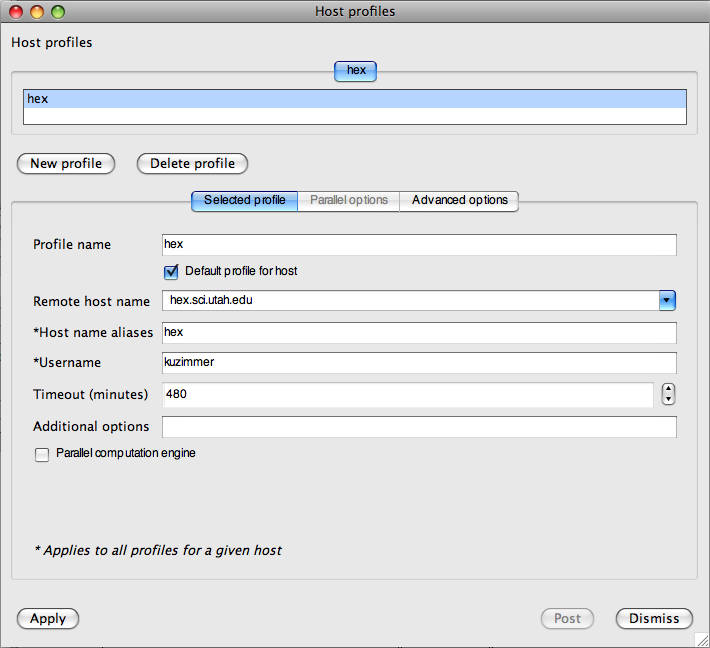
\includegraphics[width=.425\textwidth]{VisItHostProfile.png}
  \end{center}
   \vspace{-10pt}
  \caption{Setting up Host Profile}
   \vspace{-20pt}
  \label{VisItHostProfile}
%\end{figure}

\end{wrapfigure}

Next you will want to set up a Host Profile for your remote
machine. Select 'Host Profiles' from the 'Options' menu and set up a
new profile as shown in Figure~\ref{VisItHostProfile}.


% \begin{wrapfigure}{r}{.50\textwidth}

% %\begin{figure}
%   \vspace{-30pt}
%   \begin{center}
%     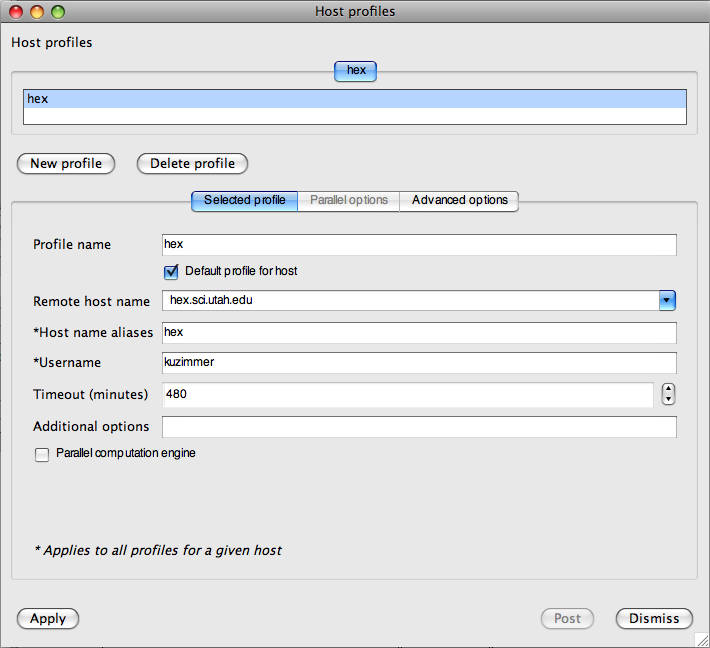
\includegraphics[width=.425\textwidth]{VisItHostProfile.png}
%   \end{center}
%   \vspace{-20pt}
%   \caption{Setting up Host Profile}
%   \vspace{-30pt}
%   \label{VisItHostProfile}
% %\end{figure}

% \end{wrapfigure}




After filling in the remote machine information, select the 'Advanced
options' tab, then 'Networking' and check the 'Tunnel data connections
through SSH' option. This is illustrated in
figure~\ref{VisItHostProfileAdv}. Click on 'Apply' and then do a 'Save
Settings' in the 'Options' menu on the gui.

% \begin{wrapfigure}{r}{.50\textwidth}

% %\begin{figure}
%   \vspace{-30pt}
%   \begin{center}
%     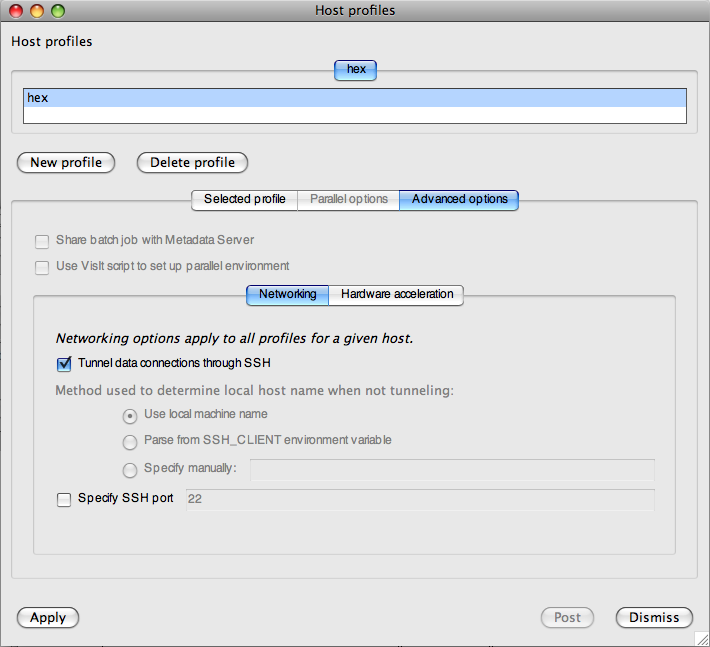
\includegraphics[width=.5\textwidth]{VisItHostProfileAdv.png}
%   \end{center}
%   \vspace{-20pt}
%   \caption{Setting up advanced options}
%   \vspace{-10pt}
%   \label{VisItHostProfileAdv}
% %\end{figure}

% \end{wrapfigure}

% \begin{wrapfigure}{r}{.50\textwidth}

% \begin{figure}

%   \begin{center}
%     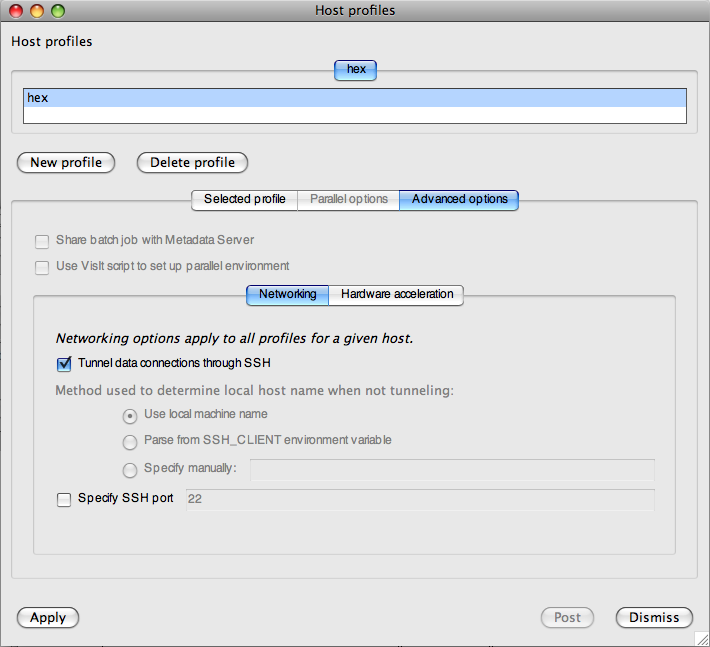
\includegraphics[width=.5\textwidth]{VisItHostProfileAdv.png}
%   \end{center}

%   \caption{Setting up advanced options}

%   \label{VisItHostProfileAdv}
% \end{figure}

% \end{wrapfigure}



For the remote visualization option to work, you must have ports 5600
- 5609 open. You can try this by running the following on your local
desktop (on Linux distributions),

\begin{verbatim}        
             traceroute -p 560[0-9] <remote machine>
\end{verbatim}

%\begin{wrapfigure}{r}{.50\textwidth}

% \begin{figure}
%   \vspace{-30pt}
%   \begin{center}
%     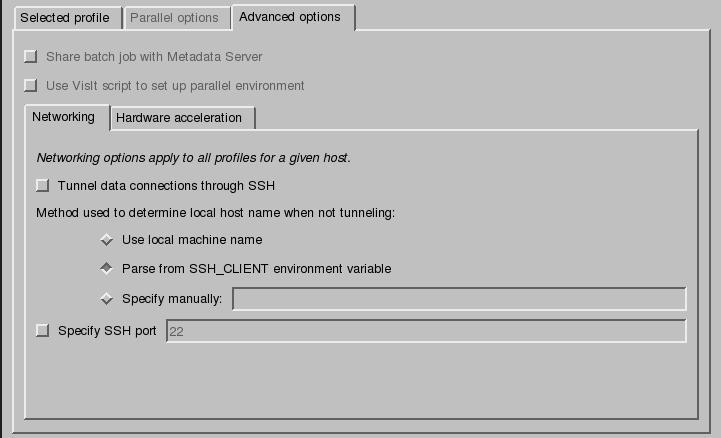
\includegraphics[width=.5\textwidth]{VisItHostProfileAdv2.png}
%   \end{center}
%   \vspace{-20pt}
%   \caption{Setting up advanced options}
%   \vspace{-10pt}
%   \label{VisItHostProfileAdv2}
% \end{figure}

%\end{wrapfigure}


\begin{figure}[h]
  \centering
  \vspace{5pt}
  \subfloat[Setting up advance options]{\label{VisItHostProfileAdv}
    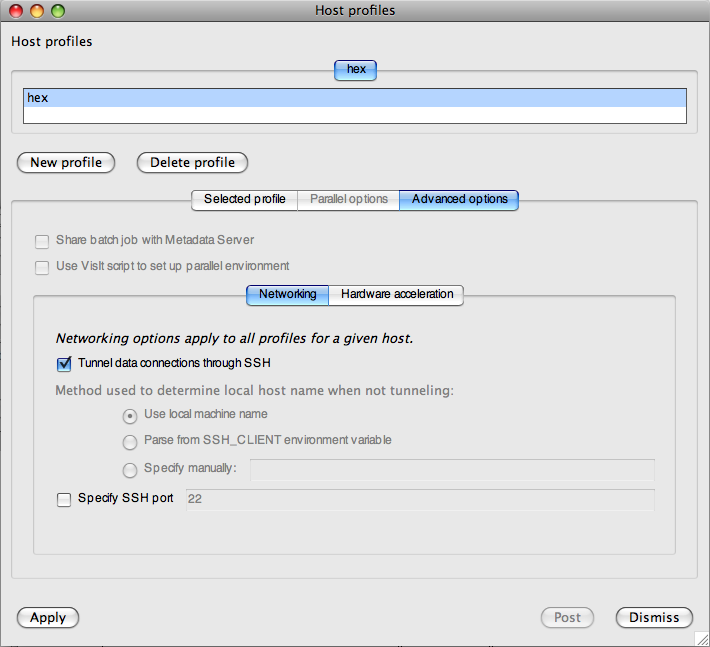
\includegraphics[width=.4\textwidth]{VisItHostProfileAdv.png}}
  \hspace{20pt}
  \qquad
  \subfloat[Setting up advance options]{\label{VisItHostProfileAdv2}
    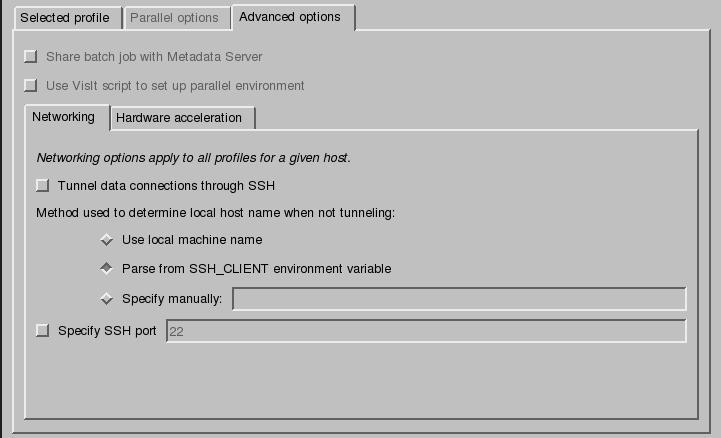
\includegraphics[width=.4\textwidth]{VisItHostProfileAdv2.png}}
  \caption{}
  \vspace{-10pt}
  \label{}
\end{figure}

If the tunneling option doesn't works, try the option as shown in
Figure~\ref{VisItHostProfileAdv2}. Now you should be able select
'Open' from VisIt's 'File' menu. After selecting your host from the
host entry list, you will be prompted for a password on the remote
machine (unless you have set up passwordless ssh access).

Once the ssh login has completed, you should see the directory
listing. You can then change directories to your UDA and load the
data.




% \section{Mac OSX Installation}

% Following are step-by-step instructions for installing the
% \textbf{Uintah Computational Framework} on \textbf{Mac OSX}.  It is
% assumed that all commands are run as administrator (which may require
% a sudo).  These instructions were tested on OSX 10.5.6 and 10.5.7 but
% should work on previous versions.  \textbf{If you have Snow Leopard,
% go to Section 10.}

% \subsection{Installing Developer Tools}
% Install the suite of developer tools that are packaged with Mac OS X.
% These can be found in the "Optional Installs" directory on the Mac OS
% X Installation CD for newer versions (i.e. Tiger, Leopard) or on the
% included Developer CD if your version of OSX is older). If you don't
% have the installation CD you can download older versions from:
% \url{http://connect.apple.com}

% Double-click the XCodeTools.mpkg and follow the installer
% instructions.  This will install GCC, as well as many other useful
% developer tools.

% \subsection{Installing Fortran Compiler}
% Download gfortran from \url{http://hpc.sourceforge.net/} making sure
% the package is designed for your CPU architecture--Intel or PowerPC.
% Put package in root directory and extract.  Extracting from / puts
% everything in the correct places.  Extract using:

% \begin{verbatim}
% 	tar -xvf gfortran-*-bin.tar.gz
% \end{verbatim}

% Note: If the Uintah builds correctly, but you are receiving link errors, see section 10.2.

% \subsection{Installing Subversion/libpng3/libxml2/other dependencies}
% As mentioned above, several libraries are required for Uintah, and may
% need to be updated or installed depending on the version of Mac
% running.  Some of these include SVN, libpng3, cmake, zlib and libxml2,
% which are all conveniently part of the fink project.

% Download the appropriate version of fink for your version of OSX from
% \url{http://www.finkproject.org/download/srcdist.php}.  Where "x" and
% "y" are version numbers, extract and install with:

% \begin{verbatim}
% 	tar -xvf fink-0.x.y-full.tar 
% 	cd fink-0.x.y-full
% 	./bootstrap 
% 	pathsetup.sh
% \end{verbatim}

% For a GUI version of fink, download Fink Commander and install from
% disk image from \url{http://finkcommander.sourceforge.net/} following
% instructions in the installer.  The Fink Commander website stresses
% that you install Commander after fink.

% Finally, update or install any necessary packages using Fink
% Commander's search bar.

% \subsection{Install/Update X11}
% X11 can be found in the "Optional Installs" directory accompanying
% your Mac OS Installation CD.  This copy should be updated.
% Alternately, X11 can be downloaded from the web and installed.
% Current versions can be found at
% \url{http://xquartz.macosforge.org/trac/wiki/Releases}.  Find a
% package that matches your version of OSX (or update OSX to newest
% version), and install it.  Installation is as simple as downloading
% the disk image from this site, mounting it, double-clicking the
% installer application, and following instructions.

% \subsection{Installing an LAM MPI}
% We recommend that you avoid using fink to install LAM MPI.
% The files and libraries are installed in non-traditional locations 
% and Uintah cannot find them. (11/10/2010) \\

% Download LAM MPI from \url{http://www.lam-mpi.org}
% version 7.1.4 or newer.  Make a new directory in \textasciitilde/ for
% this and all of the following source packages.  This documentation
% assumes this directory is \textasciitilde/Uintah.  Inside this
% directory make another for installation directories.  This
% documentation assumes this directory is
% \textasciitilde/Uintah/installs

% \begin{verbatim}
% 	cd ~/Uintah/installs
% 	tar -xvf lam-7.1.4.tar.gz
% 	cd lam-7.1.4
% 	./configure --prefix=/Users/<username>/Uintah/installs/lam-7.1.4 \
% 	            --enable-shared=yes --with-fc=gfortran
% 	make
% 	make install
% \end{verbatim}

% These last two commands will build LAM in the directory to which
% --prefix= points.

% \subsection{Installing PETSc}
% PETSc and Hypre (the next two packages to install) are used by Uintah
% for their PDE and linear algebra and capabilities respectively.
% Download PETSc from
% \url{http://www-unix.mcs.anl.gov/petsc/petsc-as/download/index.html}.
% Unarchive it in \textasciitilde/Uintah/installs directory using a
% similar tar command as is found above.  Configure using:

% \begin{verbatim}
% 	./config/configure.py \
% 	   --prefix=/Users/<username>/Uintah/installs/petsc-2.3.3-p13 \
% 	   --with-matlab=false \
% 	   --with-x=false \
% 	   --with-shared=0 \
% 	   --with-debugging=0 \
% 	   --with-mpi-dir=/Users/<username>/Uintah/installs/lam-7.1.4
% \end{verbatim}

% Set the environmental variables the configuring process asks you to
% set, and install using:

% \begin{verbatim}
% make
% make install
% \end{verbatim}

% \subsection{Installing Hypre}
% Download Hypre version 2.9.0b from
% \url{https://computation.llnl.gov/casc/hypre/software.html} to
% \textasciitilde/Uintah/installs.  Unarchive and install by running

% \begin{verbatim}
% cd hypre-2.9.0b/src
% ./configure \
%    --with-MPI-include=/Users/<username>/Uintah/installs/lam-7.1.4/include \
%    --with-MPI-lib-dirs=/Users/<username>/Uintah/installs/lam-7.1.4/lib \
%    --with-MPI-libs="mpi lam pmpi util" \
%    --prefix=/Users/<username>/Uintah/installs/hypre-2.0.0/hypre_install \
%    CFLAGS="-DMPIPP_H" \
%    CXXFLAGS="-DMPIPP_H" 
% make
% make install
% \end{verbatim}

% Take down of your --prefix line for future reference, as this is where
% you will point Uintah's configure.

% \subsection{Installing Uintah}
% Download the Uintah source from our website using:

% \begin{verbatim}
% cd ~/
% svn co https://gforge.sci.utah.edu/svn/uintah/trunk ~/Uintah
% \end{verbatim}

% Uintah will not install correctly if configured from within the source
% directory.  As such, it is advised to create a directory on the same
% level as /Uintah/src named mac[Numofbits]opt in which to configure and
% build.

% \begin{verbatim}
% cd Uintah
% mkdir mac32opt
% cd mac32opt
% ./configure \
%    --enable-optimize \
%    --with-mpi=/Users/<username>/Uintah/installs/lam-7.1.4 \
%    --with-petsc=/Users/<username>/Uintah/installs/petsc-2.3.3-p13 \
%    --with-hypre=/Users/<username>/Uintah/installs/hypre-2.0.0/hypre_install \
%    PETSC_ARCH=darwin9.3.0-c-opt \
%    F77=gfortran
% \end{verbatim}

% The previous configure command is a template, and may need editing.
% Point each of the components to the proper places and it should
% configure just fine.  If you want to build Uintah with support for
% VisIt add --with-visit=/dir/to/visit/
% Finish the process off with:

% \begin{verbatim}
% make all
% \end{verbatim}
  

% Some useful programs can be found in the installation: sus will be
% built and installed in \textasciitilde/Uintah/mac32opt/StandAlone
% Extraction utilities that extract specific variables from UDA (Uintah
% Data Archive) can be found in
% \textasciitilde/Uintah/mac32opt/StandAlone/tools

% \subsection{Installing VisIt and udaReader on Mac}

% A Mac binary distribution is available from LLNL at
% \url{https://wci.llnl.gov/codes/visit/executables.html}.  The main
% difficulty in installing Uintah with udaReader plugin has to do with
% actually finding the VisIt installation executable.  Furthermore,
% naming conventions are slightly different, and thus several links must
% be set up.

% Extract the mac install and create links by (substitute i386 and VisIt
% version where necessary):

% \begin{verbatim}
% tar xvf visit1_11_2.darwin-i386.tar.gz
% cd visit/1.11.2
% export PATHTOVISIT=\$(pwd)
% mkdir src
% ln -s \$PATHTOVISIT/darwin-i386/bin src/bin
% ln -s \$PATHTOVISIT/../bin/frontendlaucher src/bin/visit
% \end{verbatim}

% Now that the links have been set up, configure Uintah with
% --with-visit=\$PATHTOVISIT.  

% An easier solution is to download the VisIt directory from the Uintah
% source, and run xml2makefile from \$PATHTOVISIT/darwin-i386/bin on
% udareaderMTMD.xml within VisIt/udaReaderMTMD/udaREaderMTMD.xml such
% as:

% \begin{verbatim}
% xml2makefile -clobber -private VisIt/udaReaderMTMD/udaReaderMTMD.xml
% \end{verbatim}

% To install VisIt from source, see build notes for Mac inside source
% tarball.

% \subsubsection{Installing VisIt and the udaReader on a Mac running OSX 10.6.1}

% The following steps should allow one to build VisIt and the Uintah VisIt uda reader plug-in on a Macintosh running OsX 10.6.1 (Snow Leopard):
% %
% \begin{enumerate}
% \item Obtain the VisIt source from:
% \begin{verbatim}
% svn co http://portal.nersc.gov/svn/visit/trunk/src visit/src
% \end{verbatim}
% \item \begin{verbatim} cd visit/ \end{verbatim}
% \item \begin{verbatim} mkdir third-party/ \end{verbatim} (here we will compile all the third-party software needed by visit)
% \item Manually download Python.2.6.4 
% \begin{verbatim}
% http://www.python.org/
% \end{verbatim}
% to third-party/
% \item Manually download cmake 2.6.4 
% \begin{verbatim}
% http://www.cmake.org/
% \end{verbatim}
% to third-party/
% \item Manually download qt-mac-opensource-src-4.5.3 
% \begin{verbatim}
% http://get.qt.nokia.com/qt/source/qt-mac-opensource-src-4.5.3.tar.gz
% \end{verbatim}
% to third-party/
% \item Manually download VTK 5.0.0d 
% \begin{verbatim}
% http://portal.nersc.gov/svn/visit/trunk/third_party/
% \end{verbatim}
% to third-party/
% \item Inside of third-party,
% \begin{verbatim}
% cp ../src/svn-build/build_visit . 
% \end{verbatim}
% \item Execute
% \begin{verbatim}
% ./build_visit --no-visit 
% \end{verbatim}
% \item Edit the host.conf generated by build\_visit by adding: 
% \begin{verbatim}
% -D__USE_ISOC99
% \end{verbatim} 
%  to the CXXFLAGS variable. 
% \item Copy the host.conf in the third-party/ directory to ../src/config-site/ 
% \begin{verbatim}
% cp <some name>.conf ../src/config-site/
% \end{verbatim}
% \item \begin{verbatim} cd ../src/ \end{verbatim}
% \item \begin{verbatim}./configure \end{verbatim} 
% \item \begin{verbatim}make \end{verbatim}
% \item When the make fails with an error of not finding -lGLU, open databases/Shapefile/Makefile and replace -lGLU with -framework OpenGL
% \item Type make again. It should finish successfully and the VisIt executable will be in visit/src/bin
% \item Add 
% \begin{verbatim}
% #define VERSION "2.1.0"
% \end{verbatim}  
% to src/include/visit-config.h
% \item Configure Uintah with (for example): 
% \begin{verbatim}
% --with-visit=/Users/<path to visit>  
% \end{verbatim}
% \item Build Uintah
% \begin{verbatim}
% make -j# 
% \end{verbatim}
% \end{enumerate}  
%  % % % % % % % % % % % % % % % % % % % % % % % % % % % % % % % % % % % % % % % % % % % % % % % % % % % % % % % % % % % % % % % % % % % % % % % % % % % % % % % % % % % %
% \section{Mac OSX Snow Leopard Installation (10.6.3)}
% 	What follows is a working configuration for installing Uintah on Mac OSX Snow Leopard (10.6.3) under 64 bit. In this example, it is assumed that Uintah is installed under
% 	\begin{verbatim}
% 		/Users/username/uintah
% 	\end{verbatim}
% 	Also, all packages will be downloaded and installed under 
% 	\begin{verbatim}
% 		/Users/username/uintah/packages
% 	\end{verbatim}

% 	\subsection{Fink}
% 		At the time of writing of this documentation, there is no binary version of the latest Fink distribution for Mac OSX. One must compile from the source by following the instructions on the website \url{http://www.finkproject.org/download/srcdist.php}. Make sure you select 64 bit mode when prompted. Keep all other options to default.
	
% 	\subsection{gfortran}
% 		Install the binary package for gfortran from: \url{http://r.research.att.com/tools/}. Then, set the path properly. If you are using bash, this is done as:
% 		\begin{verbatim}
% 			export PATH=/usr/local/bin:$PATH
% 		\end{verbatim}
% 		Note: If the Uintah builds correctly, but you receive a dynamic link error from fortran when you try to load a uda, the links in fortran library may be pointing to the wrong place.  This can easily be fixed by navigating to the fortran library and using "otool -L" to recognize the problem, then using install\_name\_tool to fix the problem.  Both are included in the mac developer tools.
	
% 	\subsection{openmpi}
% 		Download the latest version of openmpi from: \url{http://www.open-mpi.org/}. Then configure using:
% 		\begin{verbatim}
% 			cd ~/uintah/packages
% 			tar -xvf openmpi-1.4.x
% 			cd openmpi-1.4.x
% 			./configure --prefix=/Users/username/uintah/packages/openmpi-1.4.x-install 
% 			\F77=gfortran CFLAGS=-m64 CXXFLAGS=-m64 FFLAGS=-m64
% 		\end{verbatim}
% 		Then
% 		\begin{verbatim}
% 			make
% 			make install
% 		\end{verbatim}
		
% 		\subsection{hypre}
% 		Download the latest version of Hypre from here: \url{https://computation.llnl.gov/casc/hypre/software.html}. Then, configure using:
% 		\begin{verbatim}
% 			cd ~/uintah/packages
% 			tar -xvf hypre-2.6.0b
% 			cd hypre-2.6.0b/src
% 			./configure --prefix=/Users/username/uintah/packages/hypre-2.6.0b-install 
% 												 \--with-MPI-include=/Users/username/uintah/packages/openmpi-1.4.x-install/include 
% 												 \--with-MPI-lib-dirs=/Users/username/uintah/packages/openmpi-1.4.x-install/lib 
% 												 \CC='gcc -arch x86_64' \CXX='g++ -arch x86_64' \F77='gfortran -arch x86_64' 
% 		\end{verbatim}
% 		Then
% 		\begin{verbatim}
% 			make
% 			make install
% 		\end{verbatim}
		
% 		\subsection{PETSc}
% 		For the current release of Uintah, Petsc2.3.3 or Petsc2.2.0b has been found to work well. Download the source from here: \url{http://www.mcs.anl.gov/petsc/petsc-as/download/index.html}.
% 		Then browse to the packages directory and configure as follows:
% 		{\small
% 		\begin{verbatim}
% 			cd ~/uintah/packages
% 			tar -xvf petsc-2.x.y-p15.tar.gz
% 			cd petsc-2.x.y-p15
% 			./config/configure.py \--with-shared \--with-debugging=0 
% 			\--with-mpi-include=/Users/username/uintah/packages/openmpi-1.4.x-install/include 
% 			\--with-mpi-lib=/Users/username/uintah/packages/openmpi-1.4.x-install/lib/libmpi.dylib 
% 			\--without-fortran \--prefix=/Users/username/uintah/packages/petsc-2.x.y-p15-install
% 		\end{verbatim}}
% 		Finally,
% 		{\small
% 		\begin{verbatim}
% 			PETSC_DIR=/Users/username/uintah/packages/petsc-2.x.y-p15-install; export PETSC_DIR
% 			make all test
% 			make install
% 		\end{verbatim}}
		
% 		\subsection{Uintah}
% 		Finally, create a directory in uintah
% 		{\small 
% 		\begin{verbatim}
% 			mkdir ~/uintah/mac64opt
% 		\end{verbatim}} %
% 		\noindent Now browse to the mac64opt directory and configure Uintah using the following:
% 		\emph{Note, under Mac OSX 10.6, the build has to be 64-bit.}
% 		{\small
% 		\begin{verbatim}
% 			cd ~/uintah/mac64opt
% 			../src/configure --with-mpi=/Users/username/uintah/packages/openmpi-1.4.1-install 
% 			\--with-hypre=/Users/username/uintah/packages/hypre-2.6.0b-install 
% 			\--with-petsc=/Users/username/uintah/packages/petsc-2.3.3-p15-install 
% 			\--enable-optimize='-O2' \--enable-64bit 
% 			CC=gcc CXX=g++ F77=gfortran CFLAGS=-m64 CXXFLAGS=-m64 FFLAGS=-m64
% 			PETSC_ARCH=darwin10.3.1-c-opt USE_ICE=yes USE_MPM=yes
% 		\end{verbatim}} %
% 		\noindent Finally
% 		{\small
% 		\begin{verbatim}
% 			make all
% 		\end{verbatim}}

\end{document}
